\chapter{Analiza wymagań}
Mimo iż poprzedni rozdział daje już dość klarowny obraz celu, do jakiego dążę przy projektowaniu tej biblioteki, w~niniejszym rozdziale dokonuję analizy niektórych z~wymagań. Rozpoczynam od diagramu poziomu zero~\ref{rys:use:cases}, który zawiera wszystkie najważniejsze wymagania wysokiego poziomu. Kolejne podrozdziały zawierają tekstowy opis scenariuszy. 

W~rozdziale tym starałem się nie nadużywać diagramów, gdyż ,,diagramy przypadków użycia i~związki pomiędzy przypadkami mają drugorzędne znaczenie w~procesie analizy wymagań. Przypadki użycia to dokumenty tekstowe. Tworzenie przypadków użycia sprowadza się do pisania tekstu''. Autorem tych słów jest Craig Larman, autor książki poświęconej projektowaniu oprogramowania~\cite{UML:Wzorce}.

\begin{figure}[H]
\centering
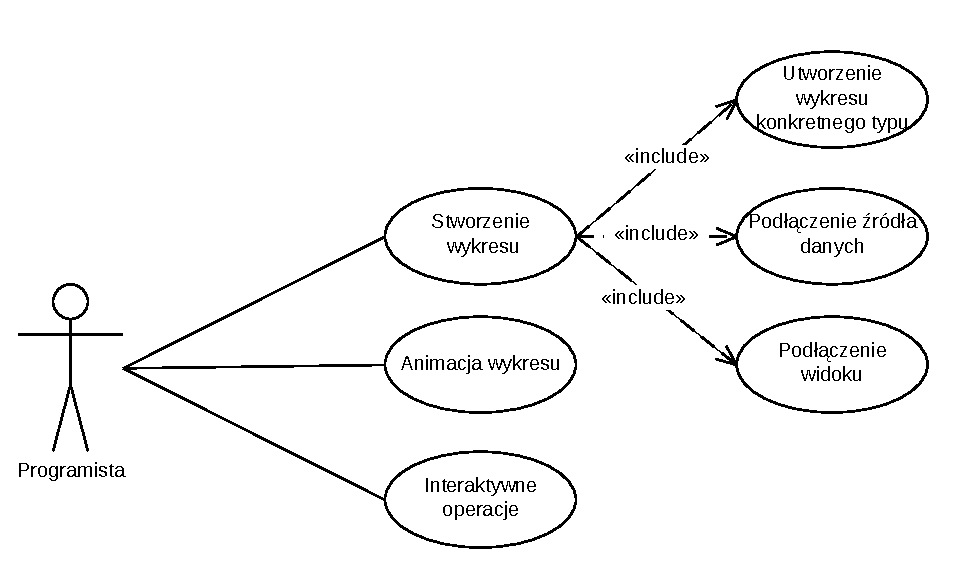
\includegraphics[scale=0.9]{img/use_case.pdf}
\caption{Diagram przypadków użycia poziomu zero}\label{rys:use:cases}
\end{figure}

\section{Stworzenie wykresu}
Stworzenie oraz wyświetlenie wykresu prezentującego dane z~określonego źródła składa się z~trzech głównych etapów, które postanowiłem opisać nieco bardziej szczegółowo.

\subsection{Utworzenie wykresu konkretnego typu}
\begin{enumerate}
\item{Programista wybiera typ wykresu i~tworzy obiekt tego typu.}
\item{Jeśli dany wykres istnieje w~kilku rodzajach, programista wybiera jeden z~nich. Wykres domyślnie przyjmuje określony rodzaj.}
\item{Programista ustawia wartości parametrów wykresu związanych z~jego odrysowywaniem, np. włączenie antyaliasingu.}
\item{Programista ustawia parametry wykresu charakterystyczne dla jego typu.}
\end{enumerate}

\subsection{Podłączenie źródła danych}
\begin{enumerate}
\item{Programista rejestruje wybrany przez siebie typ źródła danych jako \textit{QVariant}.}
\item{Programista tworzy źródło danych tego typu.}
\item{Programista wykorzystuje metodę wykresu do połączenia źródła danych z~wykresem.}
\item{Programista uzupełnia źródło danymi.}
\item{Wykres reaguje na zmianę danych poprzez ponowne odrysowanie.}
\end{enumerate}

\subsection{Podłączenie widoku}
\begin{enumerate}
\item{Programista wybiera widok, w~którym odrysowywany będzie wykres.}
\item{Programista tworzy klasę dziedziczącą po odpowiedniej klasie widoku, zgodnie z~tablicą~\ref{tab:widoki}.}
\item{Programista realizuje opisany w~rozdziale \textit{Projekt} protokół komunikacji pomiędzy widokiem a wykresem.}
\end{enumerate}


\section{Animacja wykresu}
Animacja elementów wykresu ma być możliwa poprzez wykorzystanie standardowych mechanizmów Qt.
\begin{enumerate}
\item{Programista wybiera element oraz jego właściwość, której wartość ma podlegać animacji.}
\item{Programista wybiera interesujący go typ animacji, ustawia jej parametry i~aktywuje na wybranej właściwości elementu wykresu.}
\item{Kolejne zmiany wartości właściwości powodują powiadomienie widoku wykresu o~potrzebie odrysowania.}
\item{Wykres jest odrysowywany z~uwzględnieniem zmian wynikających z~animacji.}
\end{enumerate}

\section{Interaktywne operacje}
Poniżej opisuję scenariusz potyczący dowolnej interaktywnej operacji możliwej do zaimplementowania w~ramach zaprojektowanej przeze mnie architektury.

\begin{enumerate}
\item{Programista odblokowuje daną interaktywną operację dla danej instancji wykresu.}
\item{Widok dostarcza przeznaczone dla wykresu zdarzenie.}
\item{Wykres decyduje, którego z~elementów dotyczy zdarzenie.}
\item{Wykres decyduje czy dane zdarzenie powoduje zmianę w~jego stanie, jeśli tak to podejmuje odpowiednią akcję.}
\item{Wykres powiadamia widok o potrzebie odrysowania.}
\item{Wykres jest odrysowywany z~uwzględnieniem zmian wynikających z~interakcji.}
\end{enumerate}








